\documentclass[12pt]{article}
\usepackage[letterpaper, margin=1in]{geometry}
\usepackage{graphicx}
\graphicspath{{./Figures/}}
\usepackage{hyperref}
\usepackage{parskip}
\usepackage{amsmath}
\usepackage[framed, numbered]{matlab-prettifier}
\lstset{inputpath=../MATLAB}

\title{ELECENG 3TR4 Lab 1: Fourier Analysis}
\author{
    Aaron Pinto \\ pintoa9
    \and
    Raeed Hassan \\ hassam41
}

\begin{document}

\maketitle
\clearpage

% stuff goes here
\section*{Design Problem}
The output of a function generator is a square wave with 50\% duty cycle and the period of the wave is 0.1 ms. You may assume that the amplitude of the square wave is 1 Volt. Design a second order Butterworth filter so that any harmonics in the output is at least 23 dB below the fundamental sinusoid at 10 kHz, and the loss of the fundamental sinusoid due to filtering should be less than 2 dB. The purpose of this experiment is to generate a high amplitude sinusoidal signal out of a square wave (to have a high quality sinusoid, the amplitudes of harmonics should be sufficiently low). You should choose the cutoff frequency of the filter (i.e. 3 dB bandwidth of the filter) such that the above design constraints are met.


\subsection*{Determining the Frequency Response of the Filter}
% talk about getting the frequency response of the filter (frequencyResponse.m)
The first step we took was to implement a second order Butterworth filter in MATLAB and examine its frequency response. To simulate the filter, the transfer function of a second order Butterworth filter was used. The transfer function that was used for the second order Butterworth filter was provided in the textbook.
\begin{equation*}
    H(s) = \frac{1}{s^2 + 1.414s + 1}
\end{equation*}
% how the file works
The MATLAB script used to simulate the filter, frequencyResponse.m, generated the frequency response of the filter with its transfer function using the freqs function. A portion of the MATLAB code used to generate and plot the frequency response of the filter is shown below in Listing~\ref{listing:freq_response}.
% listing
\lstinputlisting[style=Matlab-editor, caption={Generating the Frequency Response of Second Order Butterworth Filter}, label={listing:freq_response}, firstline=23, firstnumber=23, lastline=53]{frequencyResponse.m}
% how we used the file
The MATLAB script was used to visualize the normalized frequency response of the filter, and to determine the attenuation provided by the filter at frequencies of interest (the fundamental frequency, and the frequency of the third harmonic). An example of plots generated by the script is shown in Figure~\ref{fig:example_freq_response}.
\begin{figure}[h!]
    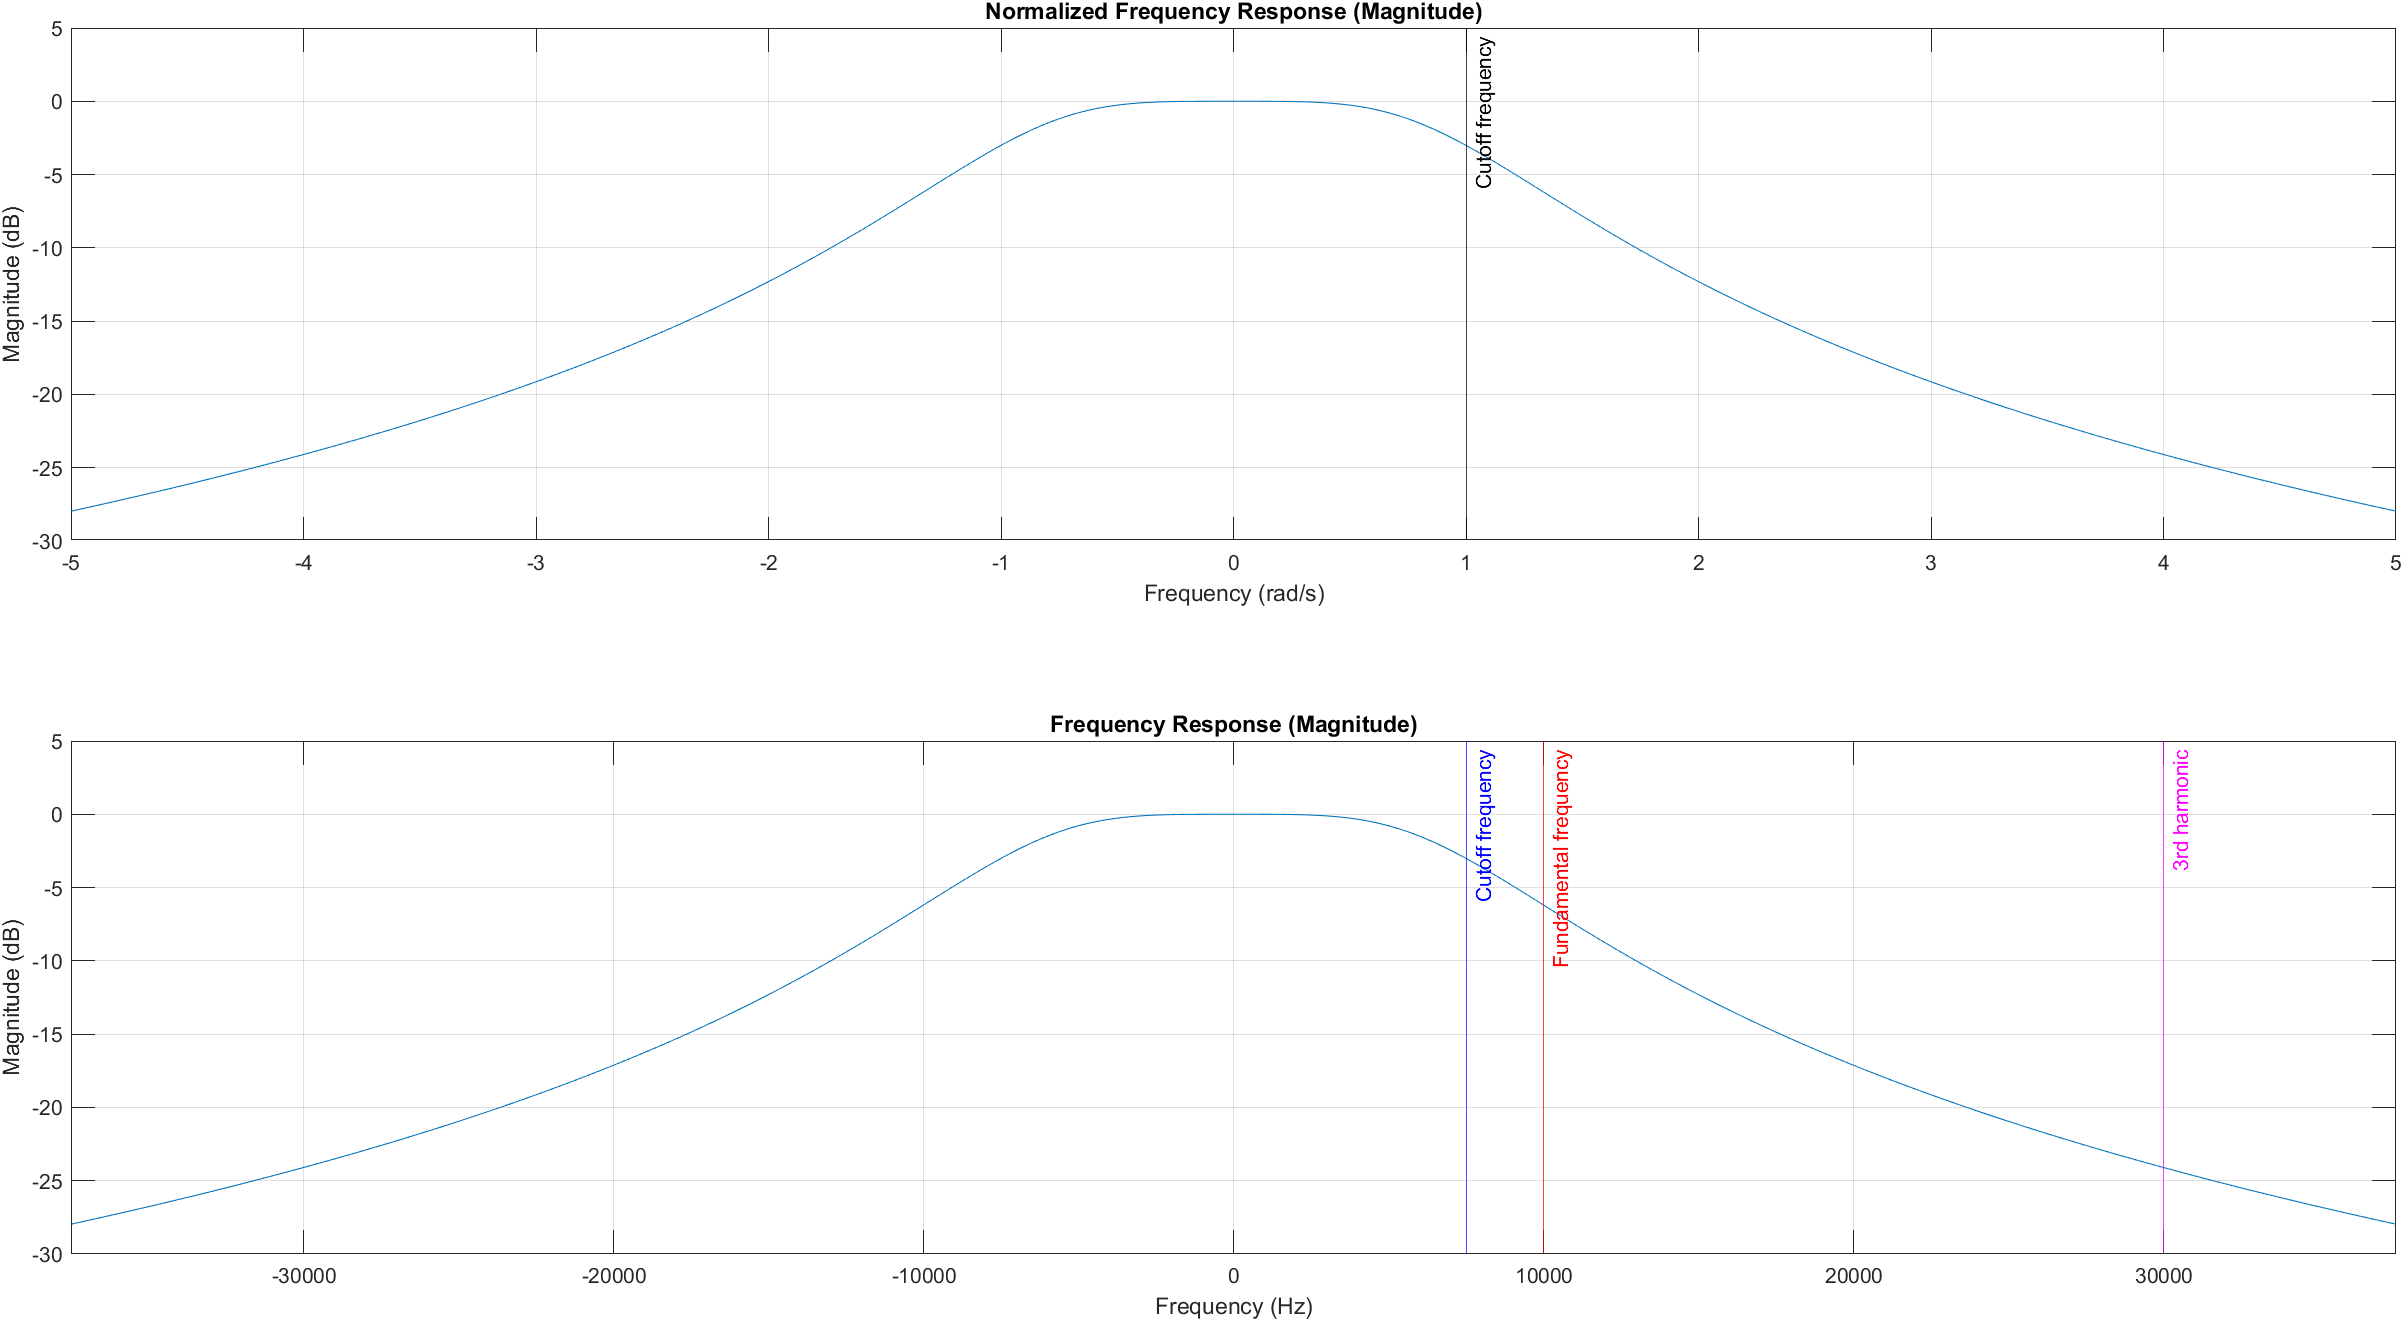
\includegraphics[width=\textwidth]{example_frequency_response.png}
    \caption{\label{fig:example_freq_response} The frequency response plots with the cutoff frequency at 7.5 kHz}
\end{figure}

\subsection*{Determining the Cutoff Frequency}
% determining minimum frequency to meet < 2 dB atten for fundamental attenuation 
The MATLAB script was used to determine the appropriate cutoff frequency to meet the design constraints. The first design constraint that we investigated required the loss of the fundamental sinusoid due to filtering to be less than 2 dB. We determined that this occurred when the cutoff frequency was greater than 11430 Hz. We selected a cutoff frequency of 11500 Hz, where the attenuation at the fundamental frequency was approximately 1.96 dB, as our starting point to continue and explore the other design constraints.

% figuring out what cutoff works for required attenuation from filter (23 - 9.54 = 13.46)
The other design constraint that had to be verified was the attenuation of harmonics other than at the fundamental frequency. The design problem requires any harmonics in the output to be at least 23 dB below the fundamental sinusoid. The square wave has natural attenuation that results the third harmonic being 9.54 dB below the first harmonic as calculated: $20\log_{10}\left(\frac{|C_3|}{|C_1|}\right) = 20\log_{10}\left(\frac{0.1061}{0.3183}\right) = -9.54$ dB. Therefore, the filter should provided an additional $23 - 9.54  = 13.46$ dB attenuation. When the cutoff frequency is 11.5 kHz, the attenuation provided by the filter is found to be approximately 14.79 dB, which is greater than the required 13.46 dB. Figure~\ref{fig:freq_response} shows the frequency response of the filter at 11.5 kHz. Therefore, we can conclude the minimum value of the cutoff frequency required to meet all design constraints is around 11.5 kHz.
\begin{figure}[h!]
    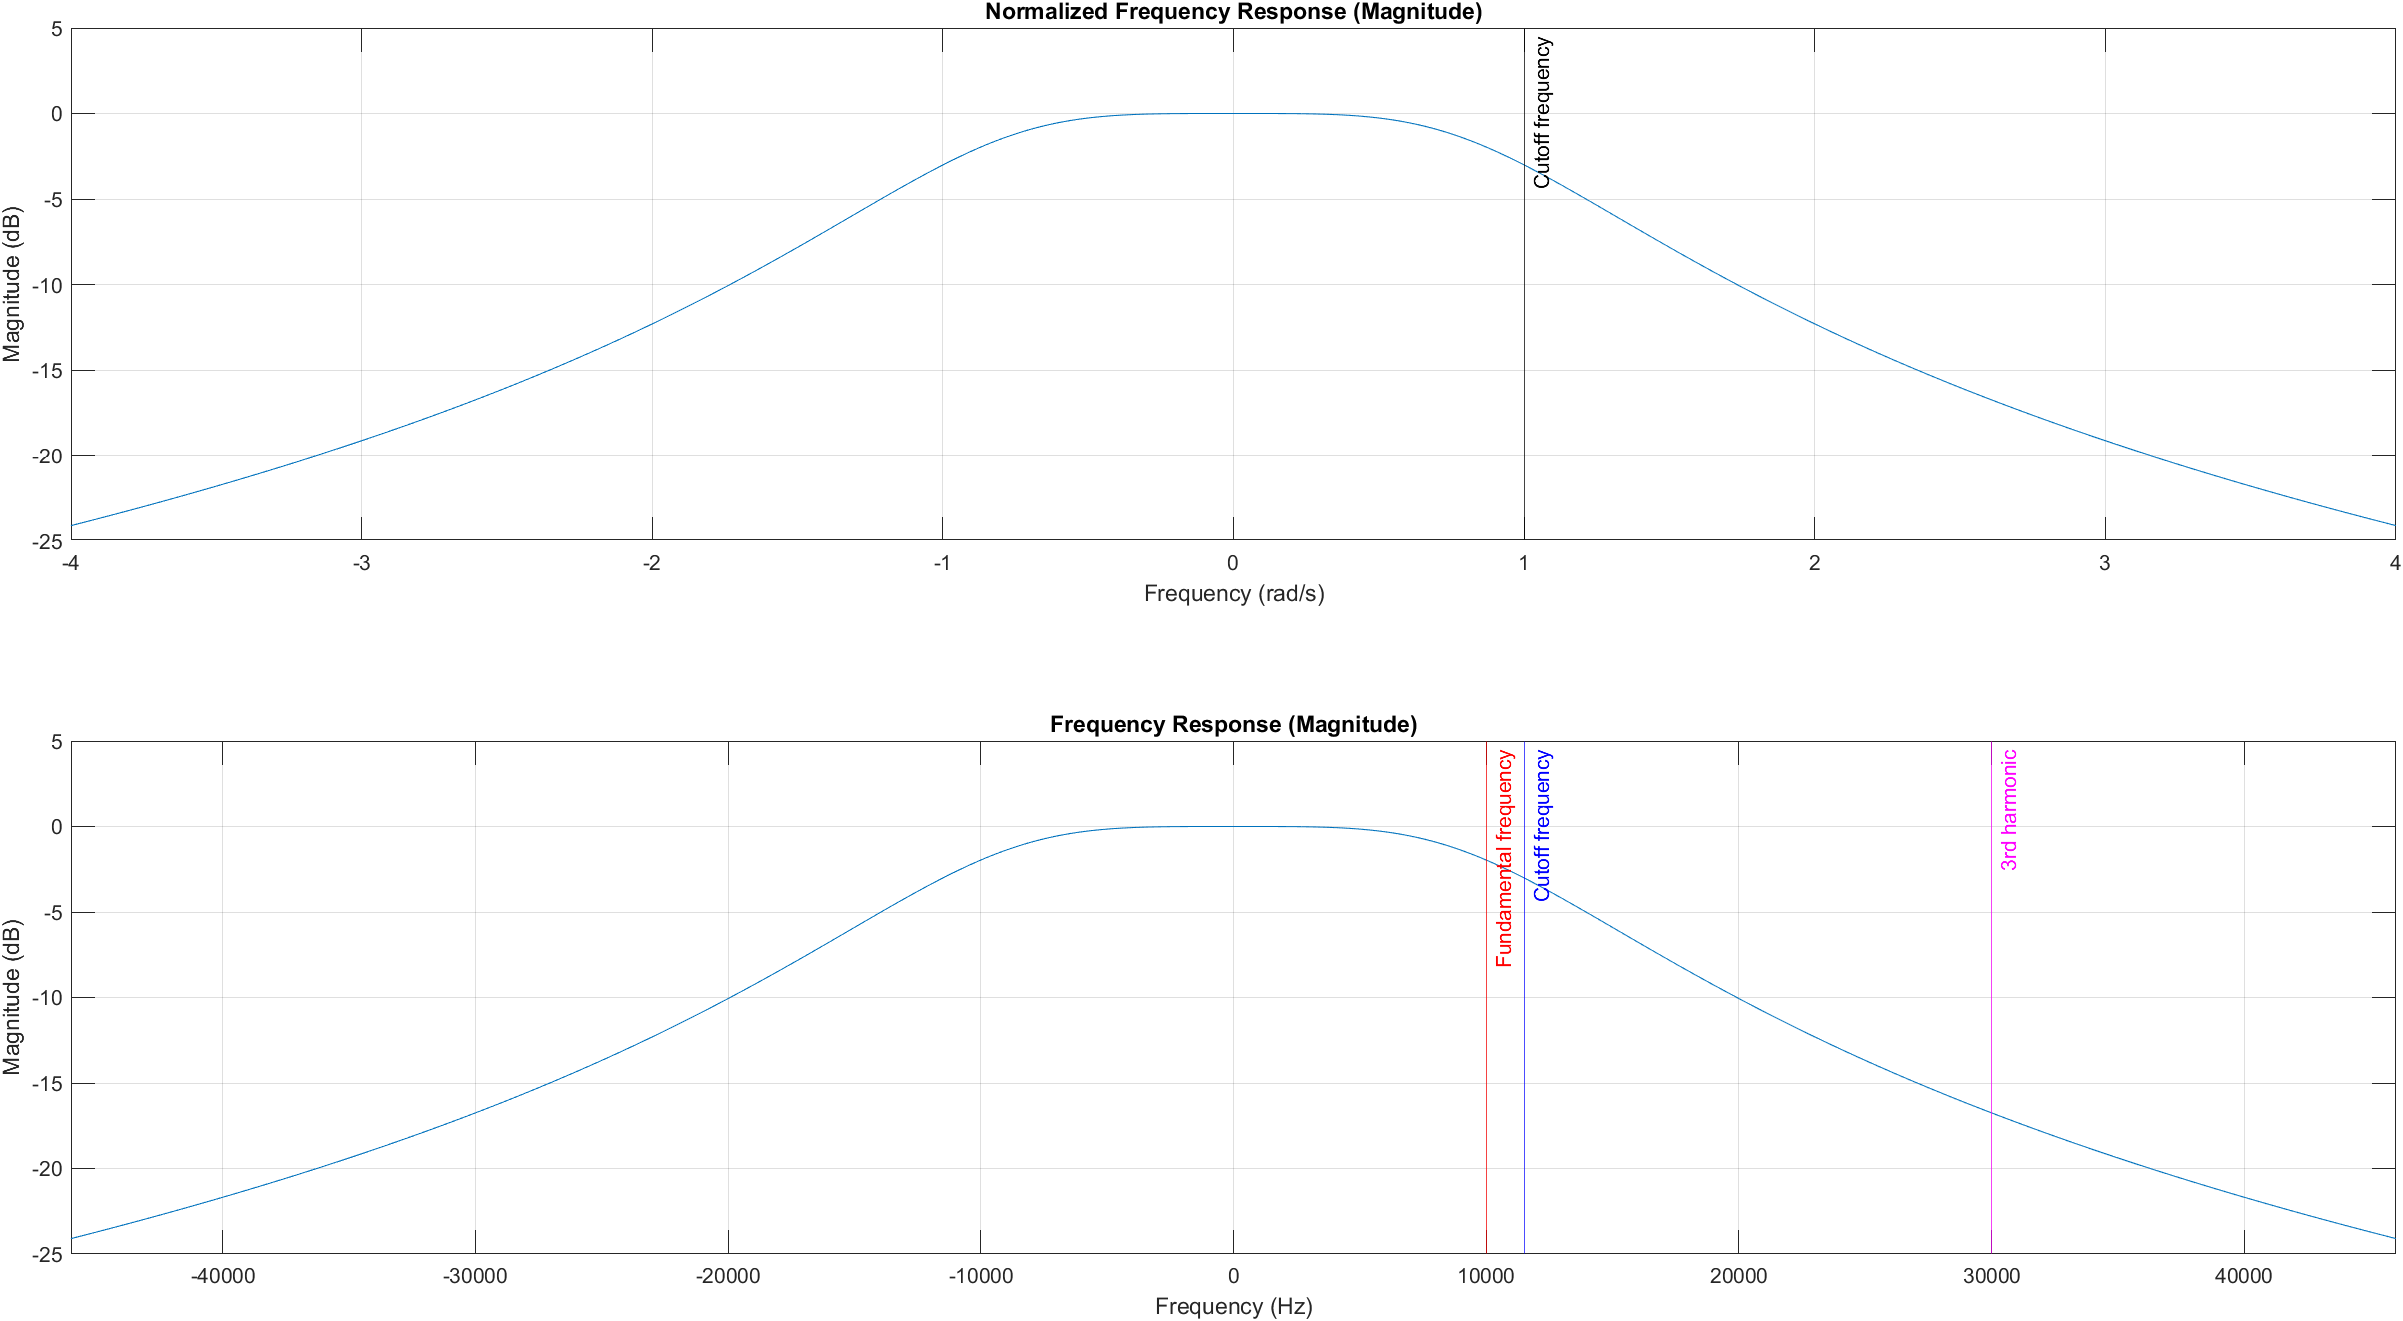
\includegraphics[width=\textwidth]{frequency_response.png}
    \caption{\label{fig:freq_response} The frequency response plots with the cutoff frequency at 11.5 kHz}
\end{figure}

\subsection*{Discussing the Impact of Changing Cutoff Frequency}
% Discuss the impact of changing the cutoff frequency on design constraints (For  example, what happens if the cutoff frequency is too large?
When increasing the cutoff frequency to be greater than 11.5 kHz, we observe that the less than 2 dB attenuation at the fundamental frequency constraint is still met, however the attenuation between the fundamental sinusoid and the third harmonic begins to decrease. Increasing the cutoff frequency too much will cause the filter to no longer provide the required attenuation between the fundamental sinusoid and other harmonics. This means that there is a maximum cutoff frequency for which the filter will still satisfy the design constraint.

% Can you satisfy the  design constraint that the any harmonic in the output is at least 25 dB below the fundamental sinusoid
When the design constraint is changed to requiring any harmonic in the output be be at least 25 dB below the fundamental sinusoid, the second order Butterworth filter is no longer sufficient to satisfy the design constraints. Any cutoff frequency that satisfies the constraint for attenuation at the fundamental sinusoid does not provide enough attenuation between the fundamental sinusoid and other harmonics in the output. To design a filter that satisfies this requirement, you will require a higher order Butterworth filter.

% higher order filter stuff
The initial design constraints can be satisfied with a second order Butterworth filter. Therefore, there is no reason to design a higher order Butterworth filter. In general, higher order Butterworth filters provide greater attenuation past the cutoff frequency, and take longer to see any attenuation before the cutoff frequency. This means that the filter could have a cutoff frequency that is much closer to the fundamental frequency, and also have a larger range of cutoff frequencies that still satisfy the design constraints. 

It is unnecessary to increase the complexity of the design as a higher order Butterworth filter would likely consume more resources in comparison to a second order Butterworth filter if it were to be implemented, despite both satisfying the design constraints.

% range of cutoff frequencies
\subsection*{Determining the Range of Acceptable Cutoff Frequencies}
We have determined through simulation that the minimum cutoff frequency required to satisfy the design constraints is around 11.5 kHz. We utilized the same approach explored earlier to determine what is the maximum cutoff frequency that the filter can use while still satisfying the design constraints, and determined that the maximum cutoff frequency is around 12.9 kHz. When the cutoff frequency is set to be greater than 12.9 kHz, the filter no longer provides the required attenuation between the fundamental sinusoid and the third harmonic. Figure~\ref{fig:max_freq_response} shows the frequency response of the filter at 12.9 kHz.

We have determined that the acceptable range of cutoff frequencies that satisfy the design constraints of the problem are between 11.5 kHz and 12.9 kHz.

% Show analytically that the filter you have designed meets the design constraints. 
We can confirm these ranges are acceptable analytically through the transfer function of the second order Butterworth filter.
\begin{equation*}
    H(s) = \frac{1}{s^2 + 1.414s + 1}
\end{equation*}
\begin{equation} \label{eq:1}
\begin{aligned}
    20\log_{10}{\left|H\left(\frac{30 \text{kHz}}{11.5 \text{kHz}}\right)\right|} - 20\log_{10}{\left|H\left(\frac{10 \text{kHz}}{11.5 \text{kHz}}\right)\right|} &\approx -16.74933 - (-1.96258) \\
    &\approx -14.79 \text{ dB}
\end{aligned}
\end{equation}
\begin{equation} \label{eq:2}
\begin{aligned}
    20\log_{10}{\left|H\left(\frac{30 \text{kHz}}{12.9 \text{kHz}}\right)\right|} - 20\log_{10}{\left|H\left(\frac{10 \text{kHz}}{12.9 \text{kHz}}\right)\right|} &\approx -14.80678 - (-1.33777) \\
    &\approx -13.47 \text{ dB}
\end{aligned}
\end{equation}

We can see through Equation~\ref{eq:1} and Equation~\ref{eq:2} that both cutoff frequencies provide the necessary attenuation from the filter $(> 13.46 \text{ dB})$ and also satisfies the condition of not having more than 2 dB of attenuation at the fundamental frequency.

\begin{figure}[h!]
    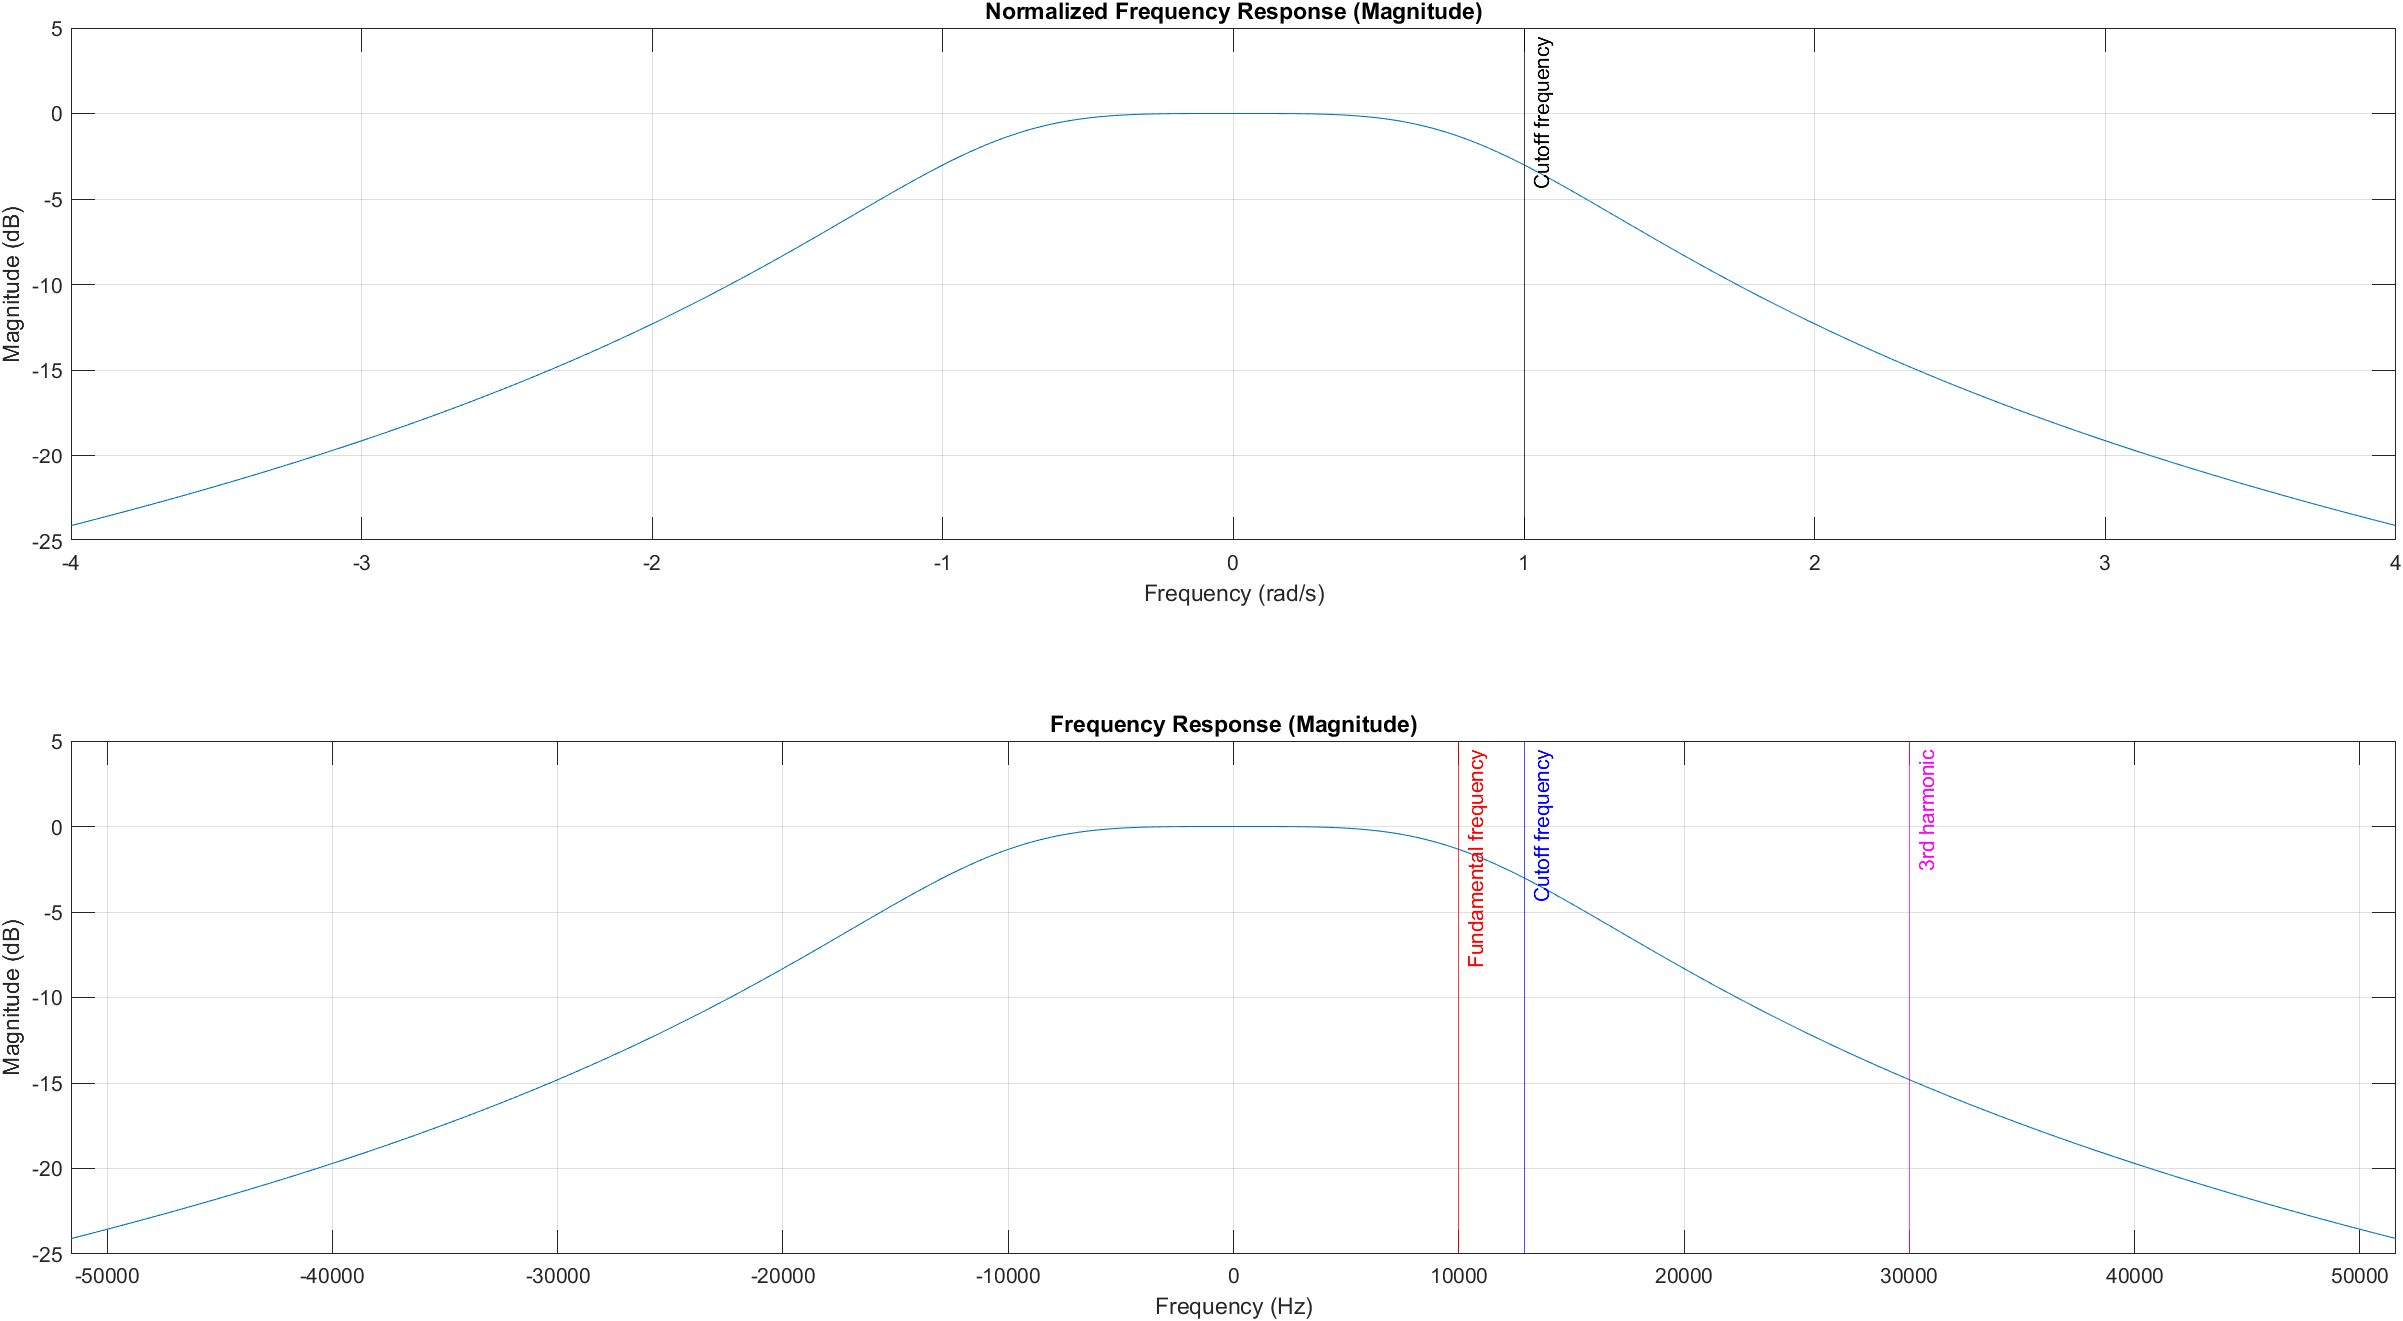
\includegraphics[width=\textwidth]{max_frequency_response.png}
    \caption{\label{fig:max_freq_response} The frequency response plots with the cutoff frequency at 12.9 kHz}
\end{figure}


\clearpage
\section*{Simulation}
The simulation of the filter was approached the same way as the triangular\_filtering.m MATLAB script provided with the lab. The MATLAB script used to simulate our filter is named lab1.m.

\subsection*{Simulating the Input}
The input of the filter is a square wave with with 50\% duty cycle, a period of 0.1 ms and an amplitude of 1 V. To generate the square wave in MATLAB, we used the square function from MATLAB's Signal Processing Toolbox. A discrete time square wave (period of 0.0001 s, amplitude of 1 V) was generated which spanned an interval of $-0.3$ ms and $0.3$ ms. The MATLAB code used to generate the square wave is shown in Listing~\ref{listing:square_wave}.
\lstinputlisting[style=Matlab-editor, caption={Generating the Square Wave}, label={listing:square_wave}, firstline=10, firstnumber=10, lastline=16]{lab1.m}

The magnitude and phase spectrums of the input signal were generated in the same manner demonstrated in the triangular filtering script. The Fourier series representation of the square wave was generated using the Fourier series coefficients of a square wave, which has been discussed previously in lecture. The magnitude spectrum plot illustrated the absolute value of the Fourier series representation, while the phase spectrum plot illustrated the angles of the Fourier series representation. The MATLAB code used to generate the magnitude and phase spectrums of the input signal is shown in Listing~\ref{listing:input_spectrum}.
\lstinputlisting[style=Matlab-editor, caption={Generating the Magnitude and Phase Spectrums of the Input}, label={listing:input_spectrum}, firstline=29, firstnumber=29, lastline=42]{lab1.m}

Figure~\ref{fig:input} shows the time and frequency domain plots of the input signal. The magnitude spectrum illustrates the magnitude of the frequency response, with an impulse at every odd harmonic (for each sinusoid that makes up the Fourier series representation of the square wave). The fundamental sinusoid (at frequency 10 kHz) contributes the most to the signal, with each subsequent sinusoid contributing a decreasing amount. These harmonics occur at every other multiple of the fundamental frequency (10 kHz, 30 kHz, 50 kHz, etc.). The phase spectrum illustrates the phase of the frequency response. % dont know what else to say about the phase
\begin{figure}[h!]
    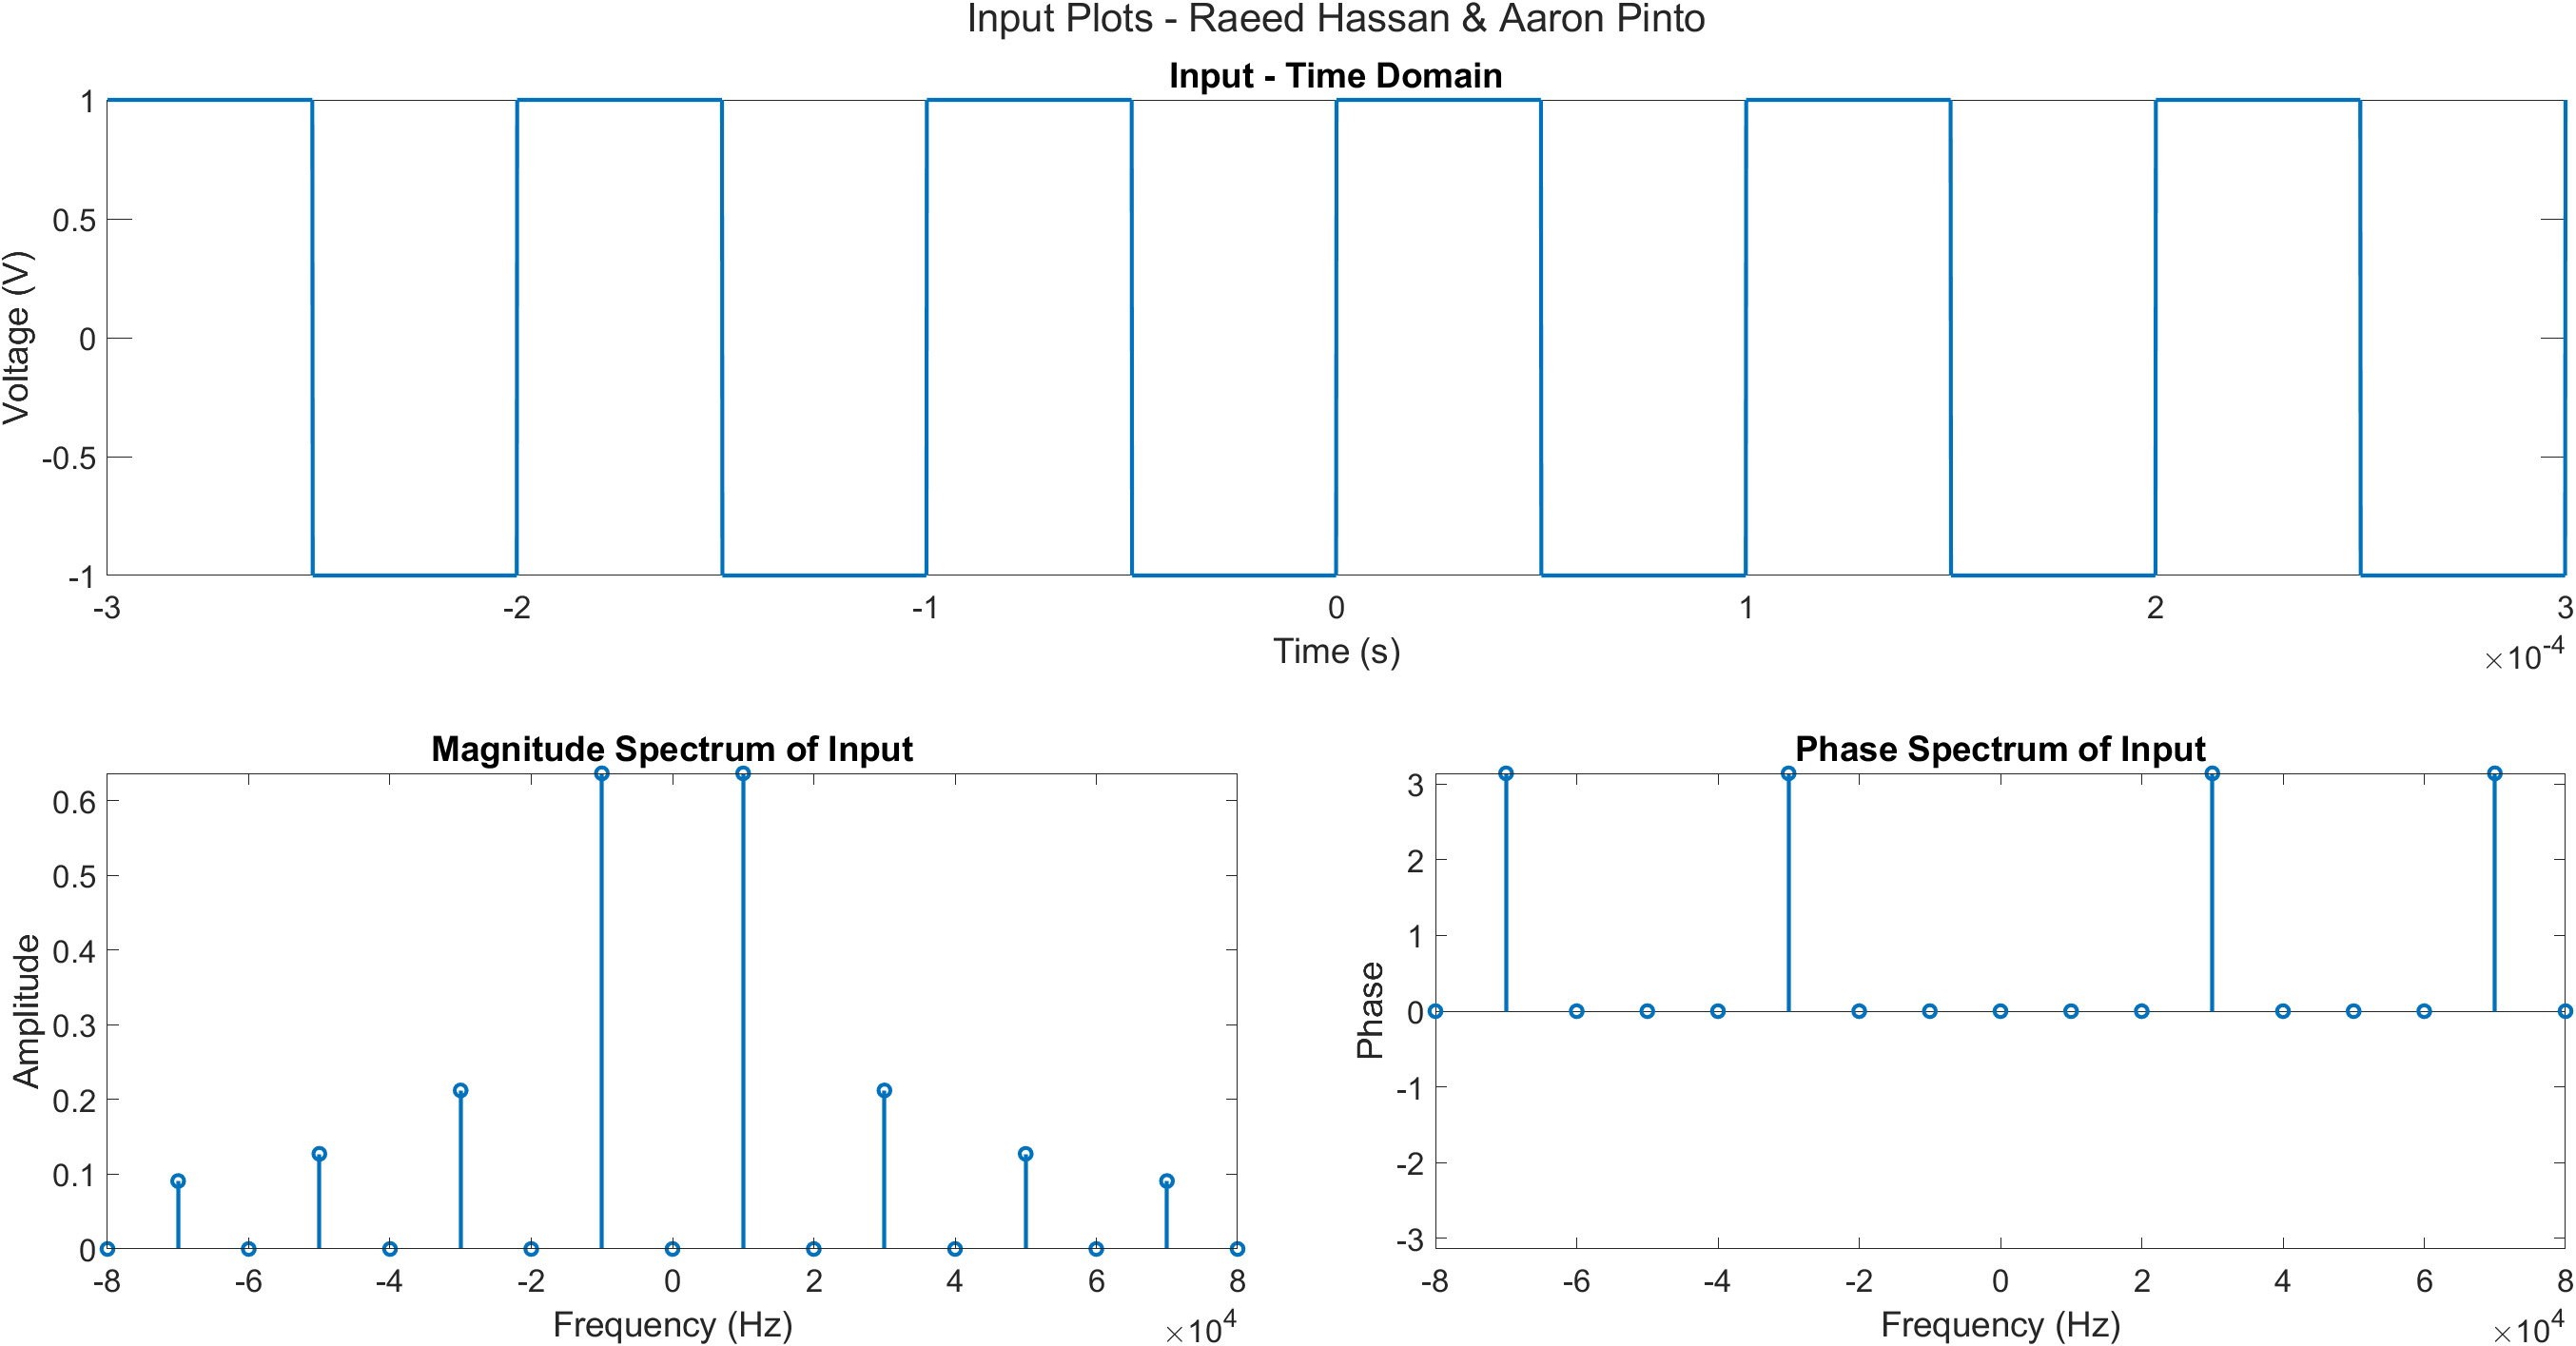
\includegraphics[width=\textwidth]{input.png}
    \caption{\label{fig:input} The time and frequency domain plots of the input signal}
\end{figure} \\

\subsection*{Simulating the Filter and the Output}
To simulate the filter and the output, we used the Fourier series representation method described in the lab document, which was also used in the provided triangular filtering file. 

The Fourier series representation of the input signal was multiplied by the transfer function evaluated at the corresponding frequencies. The cutoff frequency used when evaluating the transfer function was the minimum acceptable cutoff frequency that was previously calculated, 11.5 kHz. The magnitude and phase spectrums of the output signal was generated using this new Fourier series representation in the same manner described for the input signal. The weighted sum of the the Fourier series is calculated to generate the output signal in the time domain. The MATLAB code used to simulate the filter and the filtered output is shown in Listing~\ref{listing:filter}
\lstinputlisting[style=Matlab-editor, caption={Simulating the filter}, label={listing:filter}, firstline=69, firstnumber=69, lastline=81]{lab1.m}

The time and frequency domain plots of the output, compared with the corresponding plots of the input, are shown in Figure~\ref{fig:output}. 
\begin{figure}[h!]
    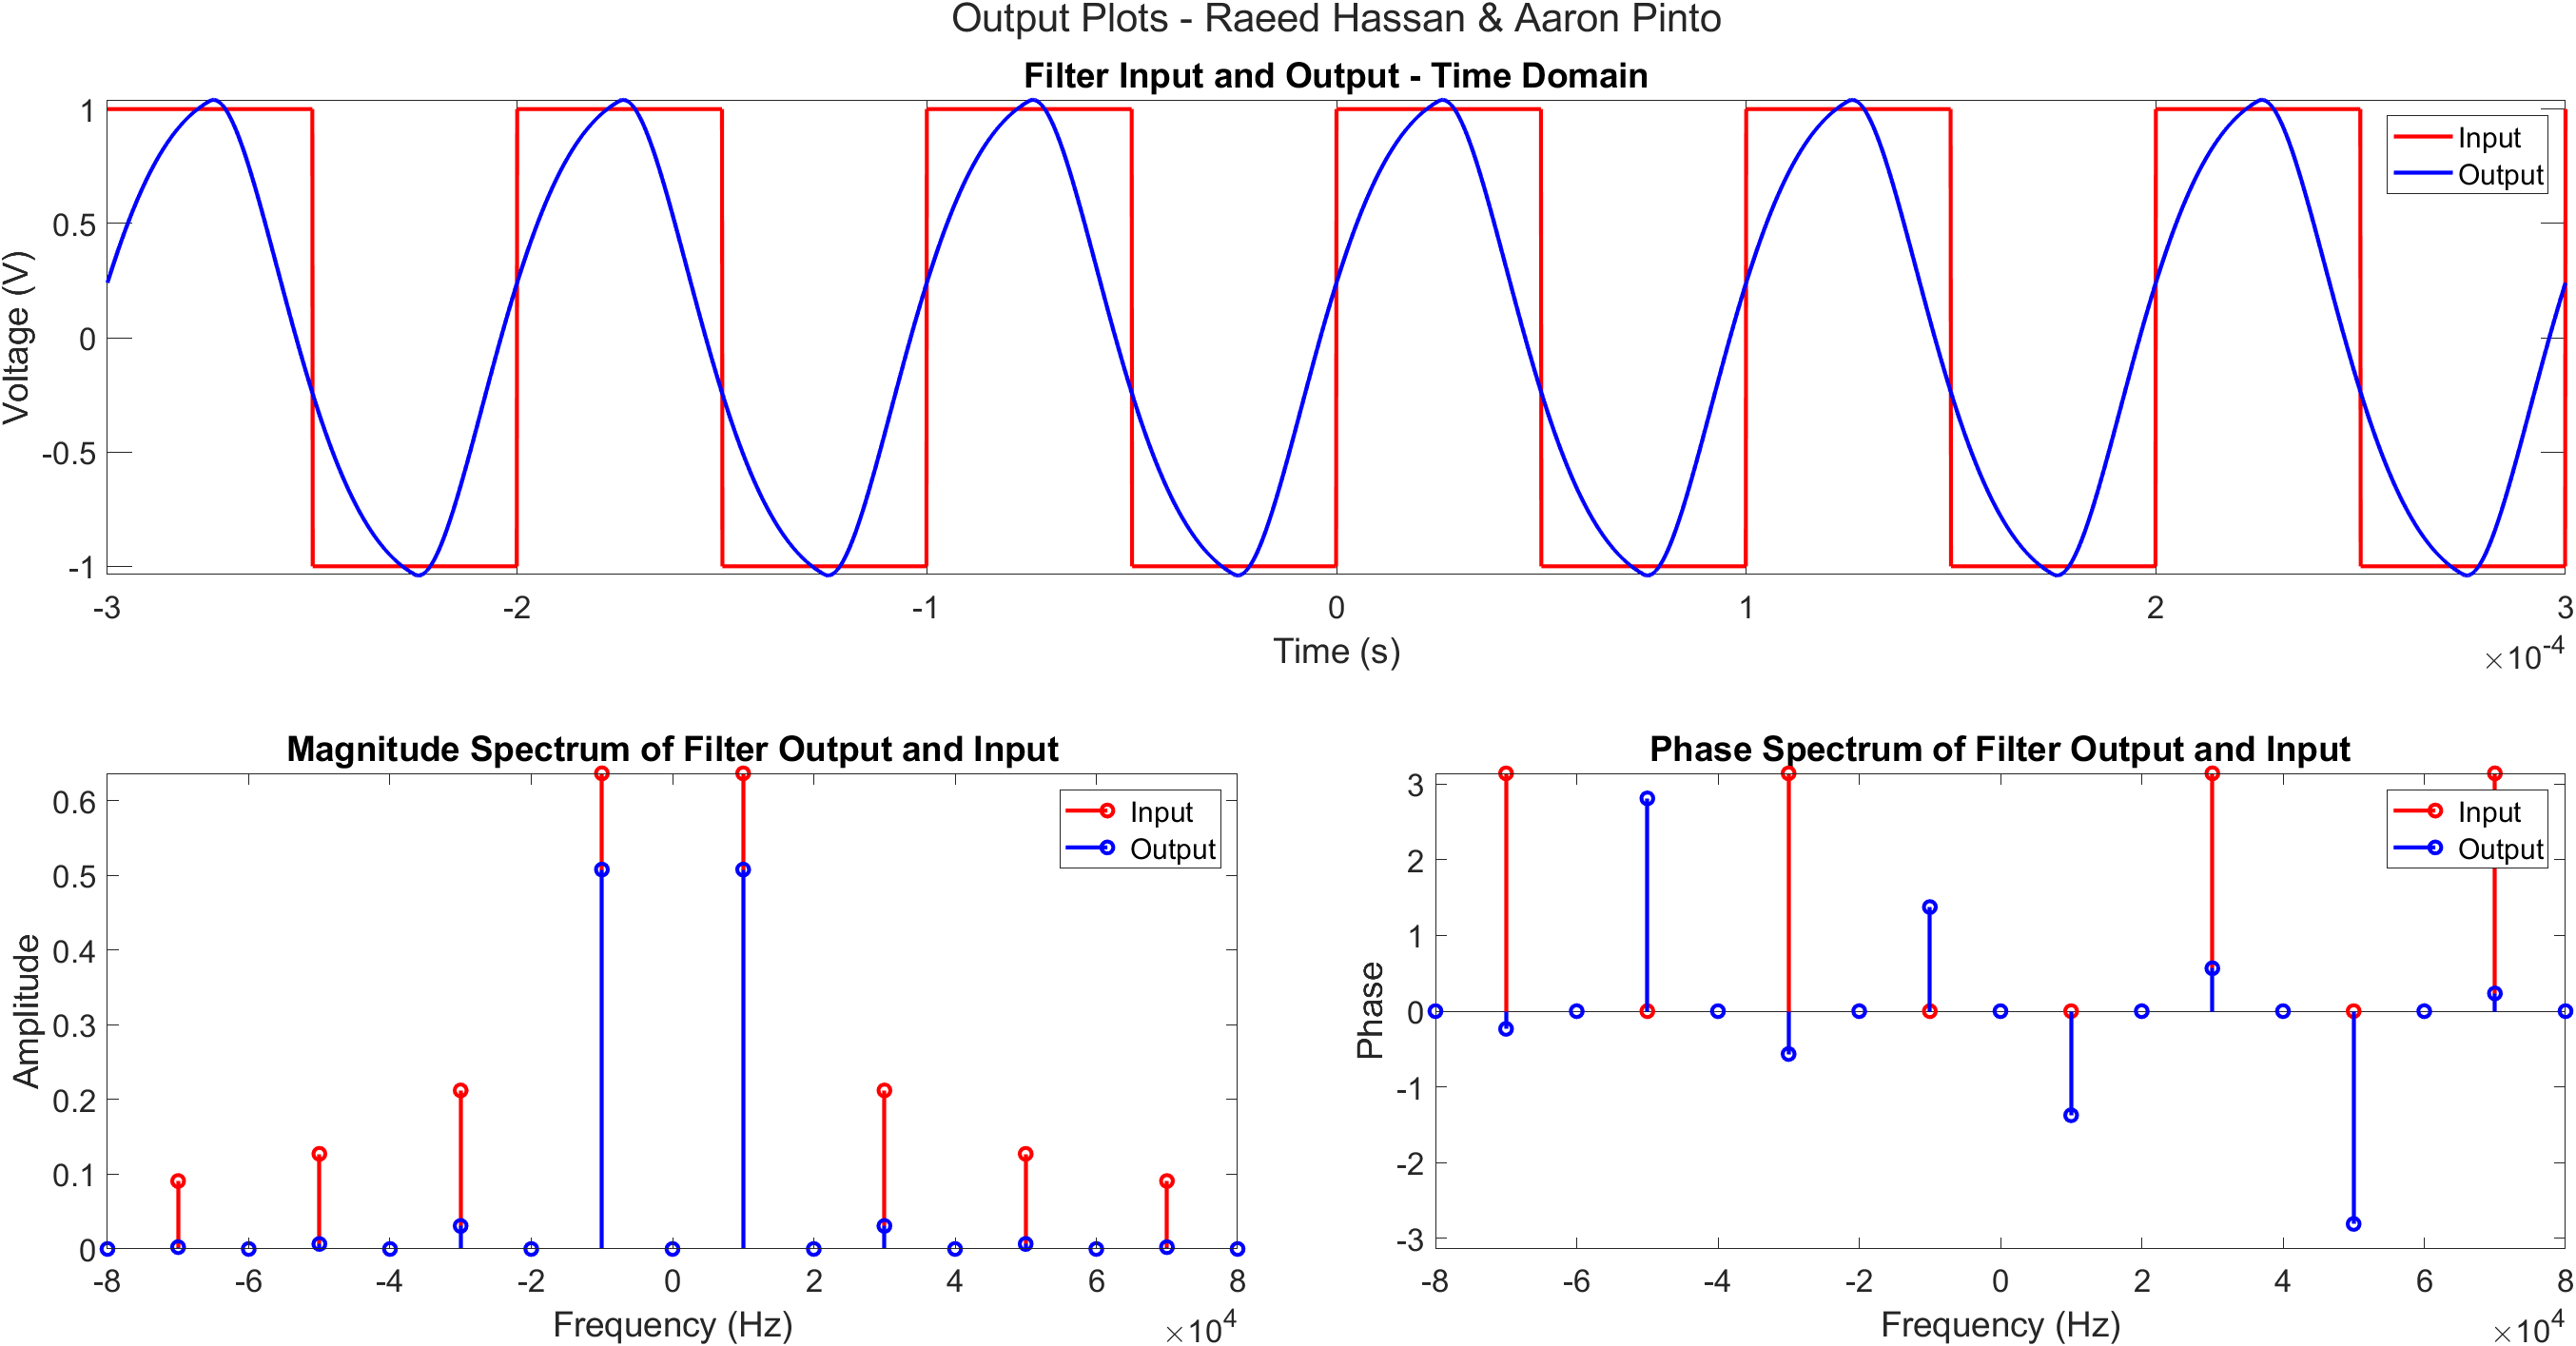
\includegraphics[width=\textwidth]{output.png}
    \caption{\label{fig:output} The time and frequency domain plots of the output signal}
\end{figure} \\
The output of the filter in the time domain closely resembles a pure sine wave with a period of 0.1 ms, which is what we were expecting at the output. All harmonics other than at the fundamental frequency have been significantly attenuated (as can bee seen in the magnitude spectrum plot), leaving the majority of the Fourier series contribution to the sinusoid at the fundamental frequency (10 kHz). An evaluation of the attenuation in the magnitude spectrum reveals that the filter satisfied the design constraints, with 1.96 dB attenuation at the fundamental frequency and 16.75 dB attenuation at the third harmonic. These values were also nearly identical to the values determined during the design process.

\clearpage
\section*{Conclusion}
In conclusion, we have determined that a second order Butterworth filter with a cutoff frequency between 11.5 kHz and 12.9 kHz will satisfy the design constraints detailed in the design problem. This was verified analytically through calculations using the filter's transfer function, and experimentally through MATLAB simulation. The MATLAB script to determine the frequency response is attached as frequencyResponse.m, and the MATLAB script used to simulate the input, filter, and output is attached as lab1.m.

\end{document}
